The communication between the CPU and GPU is handled through the high-speed serial computer expansion bus standard "Pheripheral Component Interconnect Express" more used in its abbreviation "PCI Express".

Devices connected by PCI Express communicate using a logical connection defined as a \textit{link}.
The link is a point-to-point channel, allowing both devices to send and receive PCI requests, such as configurations and memory read/writes.

A link is composed of 1, 2, 4, 8 or 16 \textit{lanes} \cite{wiki:pci}, which is furthermore composed of two differential signaling pairs, one pair for receiving data and the other for transmitting as presented on \cref{fig:hw-pci-express}.
Prior to PCI Express, the old PCI bus only allowed a single component to use the full bandwidth of the bus, as adding more devices would reduce the available bandwidth.
Lanes provide a guaranteed division of the bandwidth between all devices so that the amount of lanes used define the provided bandwidth.

\begin{figure}[ht]
	\centering
	\fbox{
		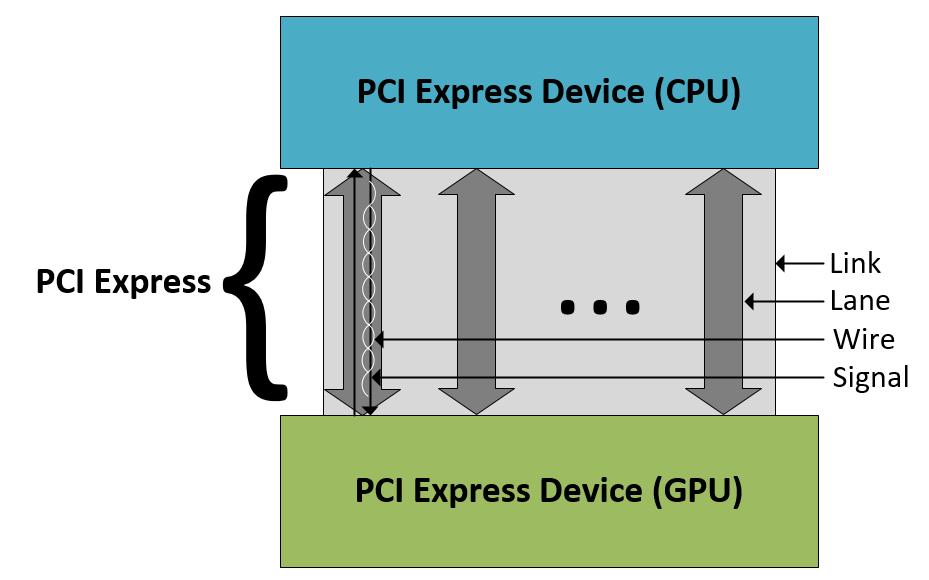
\includegraphics[width=0.6\textwidth]{figs/hw/hw-pci-express}}
	\caption{PCI Express link}
	\label{fig:hw-pci-express}
\end{figure}



As writing, PCI Express 3.x is the fastest bus version available, providing a bit rate up to 8GT/s (gigatransfers per second) equal to 985MB/s per lane.
As a single PCI Express 3.x slot can support up to 16 lanes, this results in a bit rate of up to 15.8GB/s.
The specifications for PCI Express 4.x and 5.x is however announced, with 4.x doubling the bit rate of 3.x to a total of 31.5GB/s for 16 lanes and 5.x expected to hit 63.0 or 49.2GB/s for 16 lanes \cite{wiki:pci}.

As mentioned lanes used in the bus are full-duplex, meaning that the upload speed to the GPU from the CPU is matched with the same download speed from the CPU to the GPU.
However, as the bandwidth is not cumulative, neither of the speeds will be doubled if the other is not transferring data.

PCI Express is a layered protocol, implementing layer 1, 2 and 4 of the OSI model, namely a \textit{physical layer},  a \textit{data link layer} and a \textit{transaction layer}.
% TODO: Consider extent: with OSI model
%https://web.archive.org/web/20140715120034/http://www.pcisig.com/developers/main/training_materials/get_document?doc_id=4e00a39acaa5c5a8ee44ebb07baba982e5972c67